\section{Capítulo 2 -- HTML: estrutura, semântica e acessibilidade}

O HTML é a base de toda página: é ele que diz o que cada pedaço do conteúdo \textbf{é}. Um título, um parágrafo, uma lista de ingredientes, um menu, uma tabela. Neste capítulo você vai conhecer os elementos do HTML, montar o cabeçalho completo de um documento, marcar textos, links, imagens, vídeos, listas e tabelas, e organizar a página com os elementos semânticos. No caminho, vai entender por que um HTML bem escrito é a primeira condição para que pessoas com deficiência consigam usar um site. No final, uma página de receita reúne tudo, conferida por validadores e por um verificador de acessibilidade.

\subsection{2.1 Elementos, tags e atributos}

Um documento HTML é feito de \textbf{elementos}. A maioria tem uma \textbf{tag} de abertura, um conteúdo e uma \textbf{tag} de fechamento, que repete o nome com uma barra. A tag de abertura pode trazer \textbf{atributos}, informações extras no formato \texttt{nome="valor"}:

\begin{codigo}
\begin{Verbatim}[breaklines=true, breaksymbolleft={}, fontsize=\footnotesize]
<a href="bolos.html" title="Ver todas as receitas">Bolos</a>
\_________________________________________________/\___/\__/
                         |                           |    |
        tag de abertura, com dois atributos        texto
                                                      fechamento
\end{Verbatim}
\end{codigo}

Alguns elementos não têm conteúdo nem tag de fechamento: são os \textbf{elementos vazios}, como a imagem, a quebra de linha (\texttt{<br>}) e os do cabeçalho (\texttt{<meta>}, \texttt{<link>}). E há os \textbf{comentários}, que o navegador ignora, úteis para deixar notas no código:

\begin{codigo}
\begin{Verbatim}[breaklines=true, breaksymbolleft={}, fontsize=\footnotesize]
<a href="bolos.html" title="Ver todas as receitas">Bolos</a>
<img src="img/bolo.svg" alt="Bolo de cenoura">
<!-- Um comentário: o navegador ignora, e a página não mostra -->
\end{Verbatim}
\end{codigo}

Algumas regras valem para todo o HTML:

\begin{itemize}
  \item \textbf{os elementos se aninham}, um dentro do outro, como caixas: o que abre por último fecha primeiro. \texttt{<p><strong>Olá</strong></p>} está certo; \texttt{<p><strong>Olá</p></strong>} está errado;
  \item \textbf{espaços e quebras de linha seguidos viram um espaço só}. Apertar \texttt{Enter} várias vezes no código não cria linhas em branco na página; quem cuida do espaçamento é o CSS;
  \item os nomes de tags e atributos não diferenciam maiúsculas de minúsculas, mas a convenção é escrever tudo em minúsculas;
  \item os valores dos atributos ficam entre aspas duplas.
\end{itemize}

\subsection{2.2 O cabeçalho do documento}

Todo documento HTML tem a mesma estrutura de base: a declaração do tipo, o elemento \texttt{<html>}, que envolve tudo, e, dentro dele, o \texttt{<head>}, com informações sobre a página, e o \texttt{<body>}, com o conteúdo visível. Este é o cabeçalho da página de receita que fecha este capítulo:

\begin{codigo}
\begin{Verbatim}[breaklines=true, breaksymbolleft={}, fontsize=\footnotesize]
<!DOCTYPE html>
<html lang="pt-BR">
<head>
  <meta charset="UTF-8">
  <meta name="viewport"
        content="width=device-width, initial-scale=1">
  <title>Bolo de cenoura | Receitas da Casa</title>
  <meta name="description"
        content="Bolo de cenoura com cobertura de chocolate.">
  <link rel="icon" href="favicon.svg" type="image/svg+xml">
</head>
\end{Verbatim}
\end{codigo}

\begin{center}
\begin{tabular}{@{}P{0.3\linewidth}P{0.6\linewidth}@{}}
\toprule
\rowcolor{headergray}
\tblheader{Linha} & \tblheader{Para que serve} \\
\midrule
\texttt{<!DOCTYPE html>} & diz que o documento segue o HTML atual. Sem ela, o navegador entra no ``modo de compatibilidade'' (\textit{quirks mode}) e imita defeitos de navegadores dos anos 1990 \\
\rowcolor{rowgray} \texttt{<html lang="pt-BR">} & o idioma da página: o leitor de tela pronuncia o texto em português, e o tradutor do navegador sabe de que língua partir \\
\texttt{<meta charset>} & a codificação dos caracteres; o UTF-8 representa qualquer letra de qualquer idioma, inclusive ç, ã e emojis \\
\rowcolor{rowgray} \texttt{<meta name="viewport">} & em celulares, usa a largura real da tela; sem ela, a página é desenhada com cerca de 980 pixels de largura e encolhida (Capítulo 6) \\
\texttt{<title>} & o texto da aba e do título nos resultados dos buscadores \\
\rowcolor{rowgray} \texttt{<meta name="description">} & um resumo da página, que os buscadores costumam mostrar abaixo do título \\
\texttt{<link rel="icon">} & o ícone da aba, o \textit{favicon} \\
\bottomrule
\end{tabular}
\end{center}

O \textit{favicon} resolve o erro que apareceu no Console no Capítulo 1: sem um ícone declarado, o navegador procura sozinho o arquivo \texttt{/favicon.ico}. Aqui ele é um SVG, uma imagem vetorial, que os navegadores atuais aceitam e que fica nítida em qualquer tamanho. O \texttt{<link rel="stylesheet">} e o \texttt{<script defer>}, que você viu no Capítulo 1, também ficam no \texttt{<head>}; esta página ainda não tem CSS nem JavaScript.

\subsection{2.3 Títulos e parágrafos}

O HTML tem seis níveis de título, de \texttt{<h1>} a \texttt{<h6>}. Eles formam um \textbf{sumário} da página, e é assim que leitores de tela e buscadores a entendem: o \texttt{<h1>} é o assunto da página, cada \texttt{<h2>} é uma seção dele, cada \texttt{<h3>} é uma subdivisão do \texttt{<h2>} anterior, e assim por diante. Três regras:

\begin{itemize}
  \item use um único \texttt{<h1>} por página, com o assunto principal. O padrão não proíbe mais de um, mas um só deixa o sumário claro;
  \item não pule níveis: depois de um \texttt{<h2>} vem um \texttt{<h3>}, e não um \texttt{<h4>};
  \item escolha o nível pela \textbf{hierarquia}, e nunca pelo tamanho da letra. Se o título ficou grande demais, quem muda isso é o CSS.
\end{itemize}

O \texttt{<p>} marca um parágrafo. O \texttt{<br>} força uma quebra de linha dentro dele, útil em endereços e poemas, mas não deve ser usado para criar espaço entre blocos. O \texttt{<hr>} marca uma mudança de assunto entre parágrafos e aparece como uma linha horizontal.

\subsection{2.4 Texto com significado}

Dentro de um parágrafo, alguns elementos dizem algo sobre um trecho do texto:

\begin{codigo}
\begin{Verbatim}[breaklines=true, breaksymbolleft={}, fontsize=\footnotesize]
<p>O forno deve estar <strong>preaquecido</strong>.</p>
<p>A massa fica <em>muito</em> mais fofa peneirada.</p>
<p>Use <mark>fermento químico</mark>, e não biológico.</p>
<p>O <abbr title="Instituto Nacional de Metrologia">Inmetro</abbr>
  aprova a forma.</p>
<p>Salve com <kbd>Ctrl</kbd> + <kbd>S</kbd>.</p>
<p>A função <code>alert()</code> mostra um aviso.</p>
<p>Água é H<sub>2</sub>O; a área é 10 m<sup>2</sup>.</p>
<p>Pronto às <time datetime="15:30">três e meia</time>.</p>
<blockquote cite="https://pt.wikipedia.org/wiki/Bolo">
  <p>Bolo é uma massa assada, geralmente doce.</p>
</blockquote>
<p>Como diz o ditado, <q>quem espera sempre alcança</q>.</p>
\end{Verbatim}
\end{codigo}

O \texttt{<strong>} marca algo \textbf{importante}, e o \texttt{<em>}, uma \textbf{ênfase}, que muda o sentido da frase, como a palavra ``muito''. O \texttt{<mark>} destaca um trecho, o \texttt{<abbr>} explica uma sigla no atributo \texttt{title}, o \texttt{<kbd>} representa teclas, o \texttt{<code>}, um trecho de código, e o \texttt{<sub>} e o \texttt{<sup>}, índices e expoentes. O \texttt{<time>} traz, no atributo \texttt{datetime}, a data ou a hora em um formato que programas entendem, enquanto o texto fica livre para as pessoas. O \texttt{<blockquote>} é uma citação longa, em bloco, e o \texttt{<q>}, uma citação curta, no meio da frase.

Existem também o \texttt{<b>} e o \texttt{<i>}, que, por padrão, também deixam o texto em negrito e em itálico. A diferença é o significado:

\begin{center}
\begin{tabular}{@{}P{0.2\linewidth}P{0.7\linewidth}@{}}
\toprule
\rowcolor{headergray}
\tblheader{Elemento} & \tblheader{Quando usar} \\
\midrule
\texttt{<strong>} & o trecho é importante, sério ou urgente \\
\rowcolor{rowgray} \texttt{<b>} & destaque só visual, sem importância especial, como uma palavra-chave em um resumo \\
\texttt{<em>} & ênfase, que muda o sentido da frase \\
\rowcolor{rowgray} \texttt{<i>} & uma voz diferente do texto: termos estrangeiros, nomes científicos, títulos de obras \\
\bottomrule
\end{tabular}
\end{center}

Na dúvida, prefira os que carregam significado, o \texttt{<strong>} e o \texttt{<em>}. E, para deixar um texto em negrito só porque ``fica bonito'', não use nenhum dos quatro: use o CSS.

\subsection{2.5 Links e caminhos}

O link é o elemento que fez a Web: o \texttt{<a>}, de \textit{anchor} (âncora), com o destino no atributo \texttt{href}:

\begin{codigo}
\begin{Verbatim}[breaklines=true, breaksymbolleft={}, fontsize=\footnotesize]
<a href="https://developer.mozilla.org">MDN Web Docs</a>
<a href="bolos.html">Bolos</a>
<a href="receitas/salgados.html">Salgados</a>
<a href="../index.html">Início</a>
<a href="#ingredientes">Ir para os ingredientes</a>
<a href="mailto:contato@receitas.com.br">Escreva para nós</a>
<a href="tel:+5521999990000">(21)&nbsp;99999&#8209;0000</a>
<a href="cardapio.pdf" download>Baixar o cardápio</a>
<a href="https://www.w3.org" target="_blank">W3C (nova aba)</a>
\end{Verbatim}
\end{codigo}

O destino pode ser escrito de dois jeitos. Um \textbf{endereço absoluto} é completo, com protocolo e domínio, e é usado para outros sites. Um \textbf{endereço relativo} é escrito a partir da página atual e é usado dentro do próprio site. Imagine esta estrutura de pastas:

\begin{codigo}
\begin{Verbatim}[breaklines=true, breaksymbolleft={}, fontsize=\footnotesize]
site/
  index.html
  receitas/
    bolo.html          <- a página atual
    bolos.html
    salgados.html
  img/
    bolo.svg
\end{Verbatim}
\end{codigo}

\begin{center}
\begin{tabular}{@{}P{0.38\linewidth}P{0.52\linewidth}@{}}
\toprule
\rowcolor{headergray}
\tblheader{Em \texttt{receitas/bolo.html}} & \tblheader{Aponta para} \\
\midrule
\texttt{bolos.html} & um arquivo na mesma pasta \\
\rowcolor{rowgray} \texttt{../index.html} & um arquivo na pasta de cima: \texttt{..} sobe um nível \\
\texttt{../img/bolo.svg} & sobe um nível e entra na pasta \texttt{img} \\
\rowcolor{rowgray} \texttt{/index.html} & começa pela raiz do site, de qualquer página \\
\bottomrule
\end{tabular}
\end{center}

Os endereços relativos continuam funcionando quando o site muda de domínio ou é copiado para outra pasta, por isso são a regra dentro do site. O \texttt{\#ingredientes} leva a um ponto da própria página: o elemento que tem \texttt{id="ingredientes"}. O \texttt{mailto:} abre o programa de e-mail, e o \texttt{tel:} oferece a ligação no celular. O atributo \texttt{download} pede que o arquivo seja baixado, em vez de aberto.

O \texttt{target="\_blank"} abre o link em uma nova aba. Até 2020, era preciso acrescentar \texttt{rel="noopener"} por segurança, porque a página aberta conseguia controlar a aba de origem; os navegadores atuais já aplicam essa proteção sozinhos, e o atributo só é necessário para quem precisa atender navegadores muito antigos. Use o \texttt{\_blank} com moderação: abrir abas sem pedir confunde muita gente, principalmente quem usa leitor de tela.

O texto do link deve dizer para onde ele leva, mesmo lido fora do contexto. Leitores de tela oferecem uma lista com todos os links da página, e uma lista com dez ``clique aqui'' não ajuda ninguém. Prefira ``Baixar o cardápio'' a ``Para baixar o cardápio, clique aqui''.

\subsection{2.6 Imagens}

A imagem é um elemento vazio, \texttt{<img>}, com o arquivo no atributo \texttt{src}. Na página de receita:

\begin{codigo}
\begin{Verbatim}[breaklines=true, breaksymbolleft={}, fontsize=\footnotesize]
<figure>
  <img src="img/bolo.svg" width="320" height="200"
       alt="Bolo retangular com cobertura de chocolate">
  <figcaption>O bolo pronto, ainda na forma.</figcaption>
</figure>
\end{Verbatim}
\end{codigo}

O \textbf{\texttt{alt}} é o texto alternativo: é o que o leitor de tela lê no lugar da imagem, o que aparece se ela não carregar e o que os buscadores usam para entendê-la. Ele é obrigatório, e o validador do W3C acusa a falta dele. Escreva o que a imagem \textbf{mostra} e que importa para o conteúdo: ``Bolo retangular com cobertura de chocolate'', e não ``imagem'' ou ``bolo.svg''. Se a imagem é só decorativa, como um enfeite, use \texttt{alt=""}, vazio: assim o leitor de tela sabe que pode pulá-la.

A \texttt{width} e a \texttt{height} dão o tamanho original da imagem. Com elas, o navegador reserva o espaço antes de baixá-la, e o texto não ``pula'' quando ela chega. O atributo \texttt{loading="lazy"} adia o carregamento das imagens que estão longe da área visível, até a pessoa rolar a página até elas, o que economiza dados no celular. O \texttt{<figure>} agrupa a imagem com uma legenda, o \texttt{<figcaption>}. Os formatos mais usados:

\begin{center}
\begin{tabular}{@{}P{0.18\linewidth}P{0.72\linewidth}@{}}
\toprule
\rowcolor{headergray}
\tblheader{Formato} & \tblheader{Melhor para} \\
\midrule
JPEG & fotografias \\
\rowcolor{rowgray} PNG & ilustrações, capturas de tela e imagens com transparência \\
SVG & ícones, logotipos e desenhos: é vetorial, fica nítido em qualquer tamanho e é escrito em texto \\
\rowcolor{rowgray} WebP e AVIF & os formatos modernos: a mesma qualidade do JPEG e do PNG, com arquivos bem menores \\
\bottomrule
\end{tabular}
\end{center}

\subsection{2.7 Áudio e vídeo}

O HTML toca áudio e vídeo sem nenhum programa extra:

\begin{codigo}
\begin{Verbatim}[breaklines=true, breaksymbolleft={}, fontsize=\footnotesize]
<video controls width="640" height="360" preload="metadata"
       poster="img/capa-video.jpg">
  <source src="video/preparo.webm" type="video/webm">
  <source src="video/preparo.mp4" type="video/mp4">
  <track kind="captions" src="video/preparo.vtt"
         srclang="pt" label="Português" default>
  <a href="video/preparo.mp4">Baixe o vídeo do preparo</a>.
</video>

<audio controls src="audio/dica.mp3">
  <a href="audio/dica.mp3">Ouça a dica</a>.
</audio>
\end{Verbatim}
\end{codigo}

O \texttt{controls} mostra os botões de tocar, pausar e volume. Cada \texttt{<source>} oferece o mesmo vídeo em um formato, e o navegador usa o primeiro que conseguir tocar. O \texttt{poster} é a imagem exibida antes de o vídeo começar, e o \texttt{preload="metadata"} baixa só as informações do vídeo, como a duração, até a pessoa dar o \textit{play}. O \texttt{<track>} acrescenta legendas, em um arquivo de texto no formato WebVTT: elas são indispensáveis para pessoas surdas e úteis para quem assiste sem som. O conteúdo que sobra dentro do \texttt{<video>}, o link, só aparece em navegadores que não tocam vídeo. Evite o \texttt{autoplay}: um som que começa sozinho atrapalha qualquer pessoa, e atrapalha muito quem usa leitor de tela.

\subsection{2.8 Listas}

O HTML tem três tipos de lista. A \textbf{não ordenada}, \texttt{<ul>}, é para itens em que a ordem não importa, como os ingredientes; a \textbf{ordenada}, \texttt{<ol>}, para passos em sequência, como o modo de preparo. Cada item é um \texttt{<li>}:

\begin{codigo}
\begin{Verbatim}[breaklines=true, breaksymbolleft={}, fontsize=\footnotesize]
<section>
  <h2>Ingredientes</h2>
  <ul>
    <li>3 cenouras médias</li>
    <li>3 ovos</li>
    <li>1 xícara de óleo</li>
    <li>2 xícaras de açúcar</li>
    <li>2 xícaras de farinha de trigo</li>
    <li>1 colher (sopa) de fermento em pó</li>
  </ul>
</section>

<section>
  <h2>Modo de preparo</h2>
  <ol>
    <li>Bata no liquidificador as cenouras, os ovos
      e o óleo.</li>
    <li>Misture o açúcar e a farinha, e por último
      o fermento.</li>
    <li>Asse em forno médio, a 180 °C, por cerca
      de 40 minutos.</li>
  </ol>
  <p><em>Não</em> abra o forno nos primeiros 25 minutos.</p>
</section>
\end{Verbatim}
\end{codigo}

Uma lista pode ficar dentro de um item de outra, formando sublistas. Os menus de navegação também são listas: uma lista de links, como no cabeçalho da página de receita (Seção 2.10). O leitor de tela anuncia ``lista com 6 itens'' antes de lê-los, o que ajuda a pessoa a saber o que vem pela frente. O terceiro tipo, a \textbf{lista de definições}, \texttt{<dl>}, reúne pares de termo (\texttt{<dt>}) e descrição (\texttt{<dd>}), como em um glossário:

\begin{codigo}
\begin{Verbatim}[breaklines=true, breaksymbolleft={}, fontsize=\footnotesize]
<dl>
  <dt>Banho-maria</dt>
  <dd>Cozinhar dentro de um recipiente com água quente.</dd>
  <dt>Untar</dt>
  <dd>Passar gordura na forma para a massa não grudar.</dd>
</dl>
\end{Verbatim}
\end{codigo}

\subsection{2.9 Tabelas}

Tabelas são para \textbf{dados em linhas e colunas}, em que cada célula se relaciona com o título da sua linha e o da sua coluna: notas, horários, preços, comparações. A tabela de informação nutricional da receita:

\begin{codigo}
\begin{Verbatim}[breaklines=true, breaksymbolleft={}, fontsize=\footnotesize]
<section>
  <h2>Informação nutricional</h2>
  <table>
    <caption>Valores aproximados por fatia</caption>
    <thead>
      <tr>
        <th scope="col">Item</th>
        <th scope="col">Quantidade</th>
      </tr>
    </thead>
    <tbody>
      <tr>
        <th scope="row">Calorias</th>
        <td>310 kcal</td>
      </tr>
      <tr>
        <th scope="row">Carboidratos</th>
        <td>45 g</td>
      </tr>
    </tbody>
  </table>
</section>
\end{Verbatim}
\end{codigo}

O \texttt{<caption>} é o título da tabela. O \texttt{<thead>} e o \texttt{<tbody>} separam o cabeçalho do corpo; existe também o \texttt{<tfoot>}, para totais. Cada \texttt{<tr>} é uma linha. As células de dados são \texttt{<td>}, e as de título, \texttt{<th>}, com o atributo \texttt{scope}, que diz se o título é da coluna (\texttt{col}) ou da linha (\texttt{row}). Com isso, ao chegar à célula ``310 kcal'', o leitor de tela consegue anunciar ``Calorias, Quantidade: 310 kcal''. Uma célula pode ocupar mais de uma coluna, com o \texttt{colspan}, ou mais de uma linha, com o \texttt{rowspan}:

\begin{codigo}
\begin{Verbatim}[breaklines=true, breaksymbolleft={}, fontsize=\footnotesize]
<table>
  <caption>Horário das aulas</caption>
  <thead>
    <tr>
      <th scope="col">Horário</th>
      <th scope="col">Segunda</th>
      <th scope="col">Terça</th>
    </tr>
  </thead>
  <tbody>
    <tr>
      <th scope="row">19h</th>
      <td rowspan="2">Confeitaria</td>
      <td>Massas</td>
    </tr>
    <tr>
      <th scope="row">20h</th>
      <td>Molhos</td>
    </tr>
    <tr>
      <th scope="row">21h</th>
      <td colspan="2">Prática livre</td>
    </tr>
  </tbody>
</table>
\end{Verbatim}
\end{codigo}

A ``Confeitaria'' ocupa as linhas das 19h e das 20h na segunda-feira, por isso a linha das 20h tem uma célula a menos; a ``Prática livre'' ocupa as duas colunas da linha das 21h. Nunca use tabelas para posicionar o conteúdo da página, um costume dos anos 1990: elas se comportam mal em telas pequenas e confundem os leitores de tela, que anunciam linhas e colunas que não existem. Para o layout existem o Flexbox e o Grid (Capítulo 5).

\subsection{2.10 HTML semântico}

Um HTML é \textbf{semântico} quando cada elemento foi escolhido pelo que o conteúdo \textbf{é}, e não pela aparência. Para agrupar conteúdo sem nenhum significado especial, existem o \texttt{<div>}, para blocos, e o \texttt{<span>}, para trechos dentro de uma linha, quase sempre com uma \texttt{class}, que o CSS vai usar:

\begin{codigo}
\begin{Verbatim}[breaklines=true, breaksymbolleft={}, fontsize=\footnotesize]
<div class="cartao">
  <p>Promoção: <span class="preco">R$ 15</span> a fatia.</p>
</div>
\end{Verbatim}
\end{codigo}

Eles são úteis, mas, para as grandes regiões da página, o HTML tem elementos próprios, que dizem o papel de cada uma:

\begin{center}
\begin{tabular}{@{}P{0.2\linewidth}P{0.7\linewidth}@{}}
\toprule
\rowcolor{headergray}
\tblheader{Elemento} & \tblheader{O que representa} \\
\midrule
\texttt{<header>} & o cabeçalho: o nome do site, o logotipo, a busca \\
\rowcolor{rowgray} \texttt{<nav>} & um bloco de links de navegação \\
\texttt{<main>} & o conteúdo principal da página; só um por página \\
\rowcolor{rowgray} \texttt{<article>} & um conteúdo completo em si, que faria sentido sozinho: uma receita, uma notícia, um comentário \\
\texttt{<section>} & uma seção temática, quase sempre com um título \\
\rowcolor{rowgray} \texttt{<aside>} & um conteúdo relacionado, mas à parte: dicas, anúncios, links relacionados \\
\texttt{<footer>} & o rodapé: direitos, contatos, links institucionais \\
\bottomrule
\end{tabular}
\end{center}

O começo e o fim da página de receita usam esses elementos:

\begin{codigo}
\begin{Verbatim}[breaklines=true, breaksymbolleft={}, fontsize=\footnotesize]
<header>
  <p><a href="index.html">Receitas da Casa</a></p>
  <nav aria-label="Principal">
    <ul>
      <li><a href="bolos.html">Bolos</a></li>
      <li><a href="salgados.html">Salgados</a></li>
      <li><a href="contato.html">Contato</a></li>
    </ul>
  </nav>
</header>
\end{Verbatim}
\end{codigo}

O \texttt{aria-label} dá um nome ao menu: se a página tiver mais de um \texttt{<nav>}, o leitor de tela consegue distinguir o ``Principal'' de outros. O conteúdo vem em seguida, dentro do \texttt{<main>}:

\begin{codigo}
\begin{Verbatim}[breaklines=true, breaksymbolleft={}, fontsize=\footnotesize]
<main>
  <article>
    <h1>Bolo de cenoura com cobertura de chocolate</h1>
    <p>Publicada em <time datetime="2026-10-12">12 de outubro
      de 2026</time>. Rende <strong>12 fatias</strong>.</p>
\end{Verbatim}
\end{codigo}

E, depois do artigo, a dica e o rodapé:

\begin{codigo}
\begin{Verbatim}[breaklines=true, breaksymbolleft={}, fontsize=\footnotesize]
    </article>

    <aside>
      <h2>Dica</h2>
      <p>Para a cobertura, veja a receita de
        <a href="calda.html">calda de chocolate</a>.</p>
    </aside>
  </main>

  <footer>
    <p><small>&copy; 2026 Receitas da Casa.</small></p>
  </footer>
</body>
</html>
\end{Verbatim}
\end{codigo}

Para ver a diferença que isso faz, a mesma página foi escrita do jeito errado, só com \texttt{<div>}, como ainda se encontra em sites antigos. Este é o conteúdo dela:

\begin{codigo}
\begin{Verbatim}[breaklines=true, breaksymbolleft={}, fontsize=\footnotesize]
  <div class="topo">
    <div class="logo">Receitas da Casa</div>
    <div class="menu">
      <div onclick="location.href='bolos.html'">Bolos</div>
      <div onclick="location.href='salgados.html'">Salgados</div>
    </div>
  </div>
  <div class="conteudo">
    <div class="titulo">Bolo de cenoura</div>
    <img src="img/bolo.svg" width="320" height="200">
    <div class="subtitulo">Ingredientes</div>
    <div>3 cenouras médias</div>
    <div>3 ovos</div>
  </div>
\end{Verbatim}
\end{codigo}

Na tela, com algum CSS, as duas versões poderiam ficar idênticas. Por baixo, não. As duas foram conferidas da mesma forma:

\begin{center}
\begin{tabular}{@{}P{0.32\linewidth}P{0.28\linewidth}P{0.3\linewidth}@{}}
\toprule
\rowcolor{headergray}
\tblheader{Conferência} & \tblheader{Página semântica} & \tblheader{Só com \texttt{<div>}} \\
\midrule
validador do W3C & sem erros & erro: \texttt{<img>} sem \texttt{alt} \\
\rowcolor{rowgray} verificador de acessibilidade (axe) & nenhuma violação & 4 violações \\
navegar com a tecla \texttt{Tab} & passa pelos 5 links & não chega a nenhum item do menu \\
\bottomrule
\end{tabular}
\end{center}

O último resultado é o mais grave. Quem não usa mouse navega com a tecla \texttt{Tab}, que salta de um elemento interativo para o próximo: links, botões, campos. O \texttt{<a>} é interativo por natureza; um \texttt{<div>} com \texttt{onclick} não é, e o menu simplesmente não existe para essas pessoas. As quatro violações do axe foram a imagem sem texto alternativo, a falta de um \texttt{<main>}, a falta de um \texttt{<h1>} e conteúdo fora de qualquer região da página.

\subsection{2.11 Acessibilidade}

\textbf{Acessibilidade} é a possibilidade de qualquer pessoa usar o site, inclusive pessoas cegas, que ouvem a página por um \textbf{leitor de tela}, como o NVDA, gratuito, ou o leitor que vem no celular; pessoas com baixa visão, que ampliam a tela; pessoas com deficiência motora, que usam só o teclado ou comandos de voz; pessoas surdas, que dependem de legendas; e pessoas com deficiência cognitiva, que precisam de um conteúdo claro. Segundo o Censo de 2022 do IBGE, são cerca de 14 milhões de brasileiros com algum tipo de deficiência, sem contar quem tem uma limitação temporária, como um braço quebrado, ou circunstancial, como o sol forte na tela do celular.

No Brasil, a acessibilidade dos sites é também obrigação legal: a Lei Brasileira de Inclusão (Lei n.º 13.146/2015), no artigo 63, exige sites acessíveis de empresas com sede ou representação no país e de órgãos de governo. A referência técnica internacional são as \textbf{WCAG} (\textit{Web Content Accessibility Guidelines}) do W3C, hoje na versão 2.2, e o nível que costuma ser exigido é o AA.

A boa notícia é que a maior parte da acessibilidade vem de graça com o HTML semântico. O leitor de tela não ``vê'' a página: ele percorre uma \textbf{árvore de acessibilidade}, que o navegador monta a partir do HTML, com o papel e o nome de cada elemento. Este é o começo dessa árvore para a página de receita, obtido do navegador com o Playwright, uma ferramenta que controla navegadores por código:

\begin{codigo}
\begin{Verbatim}[breaklines=true, breaksymbolleft={}, fontsize=\footnotesize]
- banner:
  - paragraph:
    - link "Receitas da Casa"
  - navigation "Principal":
    - list:
      - listitem:
        - link "Bolos"
      ...
- main:
  - article:
    - heading "Bolo de cenoura com cobertura de chocolate"
      [level=1]
    - figure "O bolo pronto, ainda na forma.":
      - img "Bolo retangular com cobertura de chocolate"
    - heading "Ingredientes" [level=2]
    - list:
      - listitem: 3 cenouras médias
      ...
\end{Verbatim}
\end{codigo}

Cada elemento semântico virou um ponto de referência com nome: \texttt{banner} é o \texttt{<header>}, \texttt{navigation} é o \texttt{<nav>}, \texttt{main}, os títulos com o seu nível, a imagem com o seu \texttt{alt}. Com isso, a pessoa pode pular direto para o conteúdo principal, ouvir a lista de títulos ou a lista de links. Para a versão só com \texttt{<div>}, a árvore inteira foi esta:

\begin{codigo}
\begin{Verbatim}[breaklines=true, breaksymbolleft={}, fontsize=\footnotesize]
- text: Receitas da Casa Bolos Salgados Bolo de cenoura
- img
- text: Ingredientes 3 cenouras médias 3 ovos
\end{Verbatim}
\end{codigo}

Um texto corrido, sem títulos, sem menu e com uma imagem sem nome. Uma lista do que conferir em toda página:

\begin{itemize}
  \item o idioma no \texttt{<html lang>};
  \item um \texttt{<h1>} e títulos em ordem, sem pular níveis;
  \item as regiões marcadas: \texttt{<header>}, \texttt{<nav>}, \texttt{<main>}, \texttt{<footer>};
  \item texto alternativo em todas as imagens, vazio nas decorativas;
  \item links com texto que diz o destino;
  \item tudo o que é clicável feito com \texttt{<a>} ou \texttt{<button>}, e alcançável pelo teclado;
  \item legendas nos vídeos;
  \item contraste suficiente entre texto e fundo (Capítulo 4).
\end{itemize}

Existem também os atributos \textbf{ARIA}, como o \texttt{aria-label} do menu, que acrescentam informações à árvore de acessibilidade. A primeira regra para usá-los, escrita pelo próprio W3C, é: se existe um elemento HTML que faz o que você precisa, use o elemento, e não o ARIA. Um \texttt{<button>} já é um botão para todos; um \texttt{<div role="button">} precisa de muito trabalho extra para chegar perto disso. Para conferir uma página, a extensão \textbf{axe DevTools}, gratuita, e a aba \textbf{Lighthouse} das ferramentas de desenvolvedor do Chrome apontam os problemas mais comuns. Elas encontram parte dos problemas, mas não todos: vale também navegar pela página só com o teclado.

\subsection{2.12 Caracteres especiais}

Alguns caracteres têm significado no HTML, como o \texttt{<}, que abre uma tag. Para mostrá-los no texto, usam-se as \textbf{entidades}, que começam com \texttt{\&} e terminam com \texttt{;}:

\begin{codigo}
\begin{Verbatim}[breaklines=true, breaksymbolleft={}, fontsize=\footnotesize]
<p>Use &lt;p&gt; para parágrafos.</p>
<p>Arroz &amp; feijão custam R$&nbsp;20.</p>
<p>&copy; 2026 &mdash; todos os direitos reservados.</p>
\end{Verbatim}
\end{codigo}

\begin{center}
\begin{tabular}{@{}P{0.22\linewidth}P{0.16\linewidth}P{0.52\linewidth}@{}}
\toprule
\rowcolor{headergray}
\tblheader{Entidade} & \tblheader{Mostra} & \tblheader{Uso} \\
\midrule
\texttt{\&lt;} e \texttt{\&gt;} & \texttt{<} e \texttt{>} & mostrar código HTML no texto \\
\rowcolor{rowgray} \texttt{\&amp;} & \texttt{\&} & o ``e comercial'' \\
\texttt{\&nbsp;} & (espaço) & um espaço que não quebra a linha, como entre ``R\$'' e o valor \\
\rowcolor{rowgray} \texttt{\&copy;} & © & o símbolo de direitos autorais \\
\texttt{\&mdash;} & — & o travessão \\
\bottomrule
\end{tabular}
\end{center}

Com o UTF-8, letras acentuadas e símbolos como © podem ser digitados diretamente; as entidades são necessárias mesmo só para o \texttt{<}, o \texttt{>}, o \texttt{\&} e os caracteres invisíveis, como o espaço que não quebra. Também existem entidades numéricas, pelo código do caractere: o \texttt{\&\#8209;} é um hífen que não quebra a linha. O html-validate pediu os dois no link de telefone da Seção 2.5, \texttt{(21)\&nbsp;99999\&\#8209;0000}, para que o número nunca seja partido entre duas linhas.

\subsection{2.13 A página completa}

Juntando os blocos das seções anteriores, a página de receita fica assim no navegador, ainda sem nenhum CSS, só com o estilo padrão:

\begin{center}
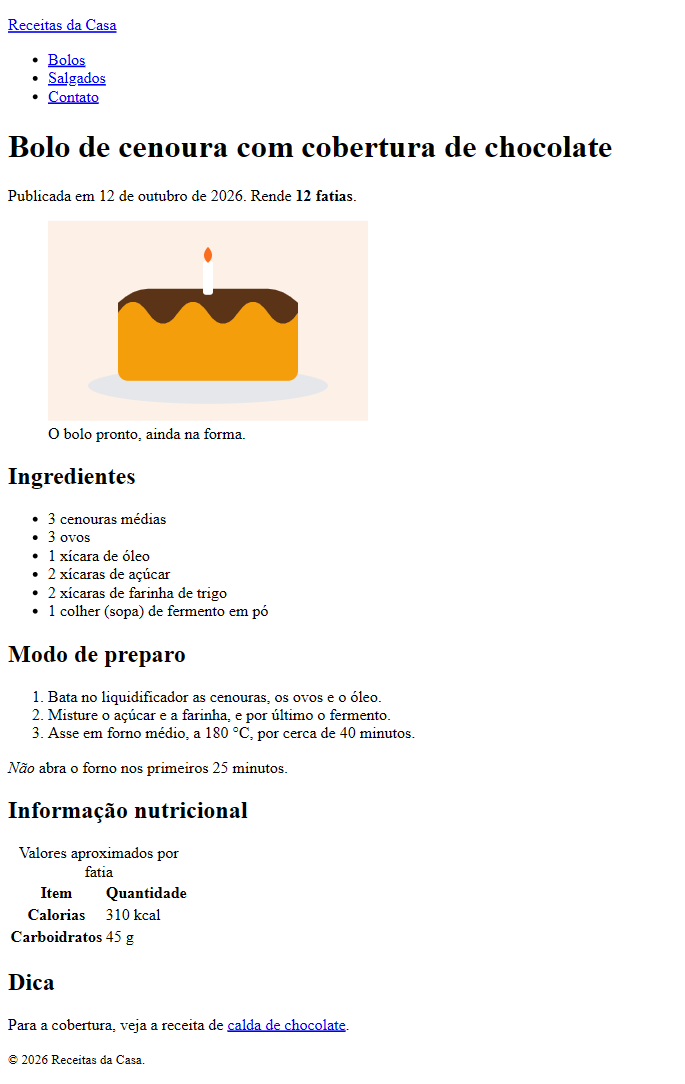
\includegraphics[width=0.6\linewidth,keepaspectratio]{imagens/capitulo-02_receita.png}
\end{center}

O navegador já dá alguma forma à página: títulos maiores, marcadores nas listas, números no modo de preparo, links sublinhados. Isso é o estilo padrão, que cada navegador aplica, e que o CSS vai substituir a partir do Capítulo 4. A página foi conferida pelos dois validadores, o do W3C e o html-validate, sem nenhum erro; pelo axe, sem nenhuma violação; e pela navegação com o teclado. O navegador baixou o HTML, a imagem do bolo e o \textit{favicon}, todos com o status \texttt{200}.

\subsection{Erros Comuns}

\begin{itemize}
  \item \textbf{Esquecer o \texttt{alt} das imagens.} A imagem some para quem usa leitor de tela. Descreva o que ela mostra, ou use \texttt{alt=""} se for decorativa.
  \item \textbf{Escolher o título pelo tamanho da letra.} Os níveis de título formam o sumário da página. Escolha pela hierarquia e ajuste o tamanho com o CSS.
  \item \textbf{Fazer botões e menus com \texttt{<div>}.} Eles não recebem o foco do teclado nem são anunciados como clicáveis. Use \texttt{<a>} e \texttt{<button>}.
  \item \textbf{Fechar os elementos fora de ordem.} \texttt{<p><strong>...</p></strong>} confunde o navegador. Feche primeiro o que abriu por último.
  \item \textbf{Usar \texttt{<br>} para dar espaço.} O espaçamento é trabalho do CSS.
  \item \textbf{Usar tabelas para posicionar a página.} Tabelas são para dados; o layout é feito com Flexbox e Grid.
  \item \textbf{Links com ``clique aqui''.} Fora de contexto, o texto não diz nada. Escreva o destino.
  \item \textbf{Esquecer o \texttt{lang} e o \texttt{charset}.} O leitor de tela lê com o sotaque errado, e os acentos podem virar símbolos estranhos.
  \item \textbf{Confiar só no que aparece na tela.} Uma página pode parecer certa e ter erros. Passe pelo validador e pelo verificador de acessibilidade.
\end{itemize}
